%----------------------------------------------------------------------------------------
%	GOALS
%----------------------------------------------------------------------------------------

\section{Konzeption des Prototyps}

%------------------------------------------------

\subsection{Datenmodellierung}

Die zentrale Datenstruktur der Applikation ist die Beschreibung der API selbst, welche als Grundlage für alle Operationen verwendet wird. Da sich der Prototyp beim Eingabeformat auf das OpenAPI Spezifikationsformat beschränkt, wurde zunächst ein graphisches Metamodell erstellt, welches in Abbildung \ref{fig:openapi} dargestellt ist. Dieses Modell wird von der Applikation als Basis-Datenstruktur verwendet. Zur Unterstützung mehrerer Eingabeformate müssten in einer späteren Iteration auch andere Spezifikationsformate untersucht werden, um Gemeinsamkeiten abzuleiten und ein Datenmodell zu erstellen in das alle Formate überführt werden können. \\

\begin{figure}
  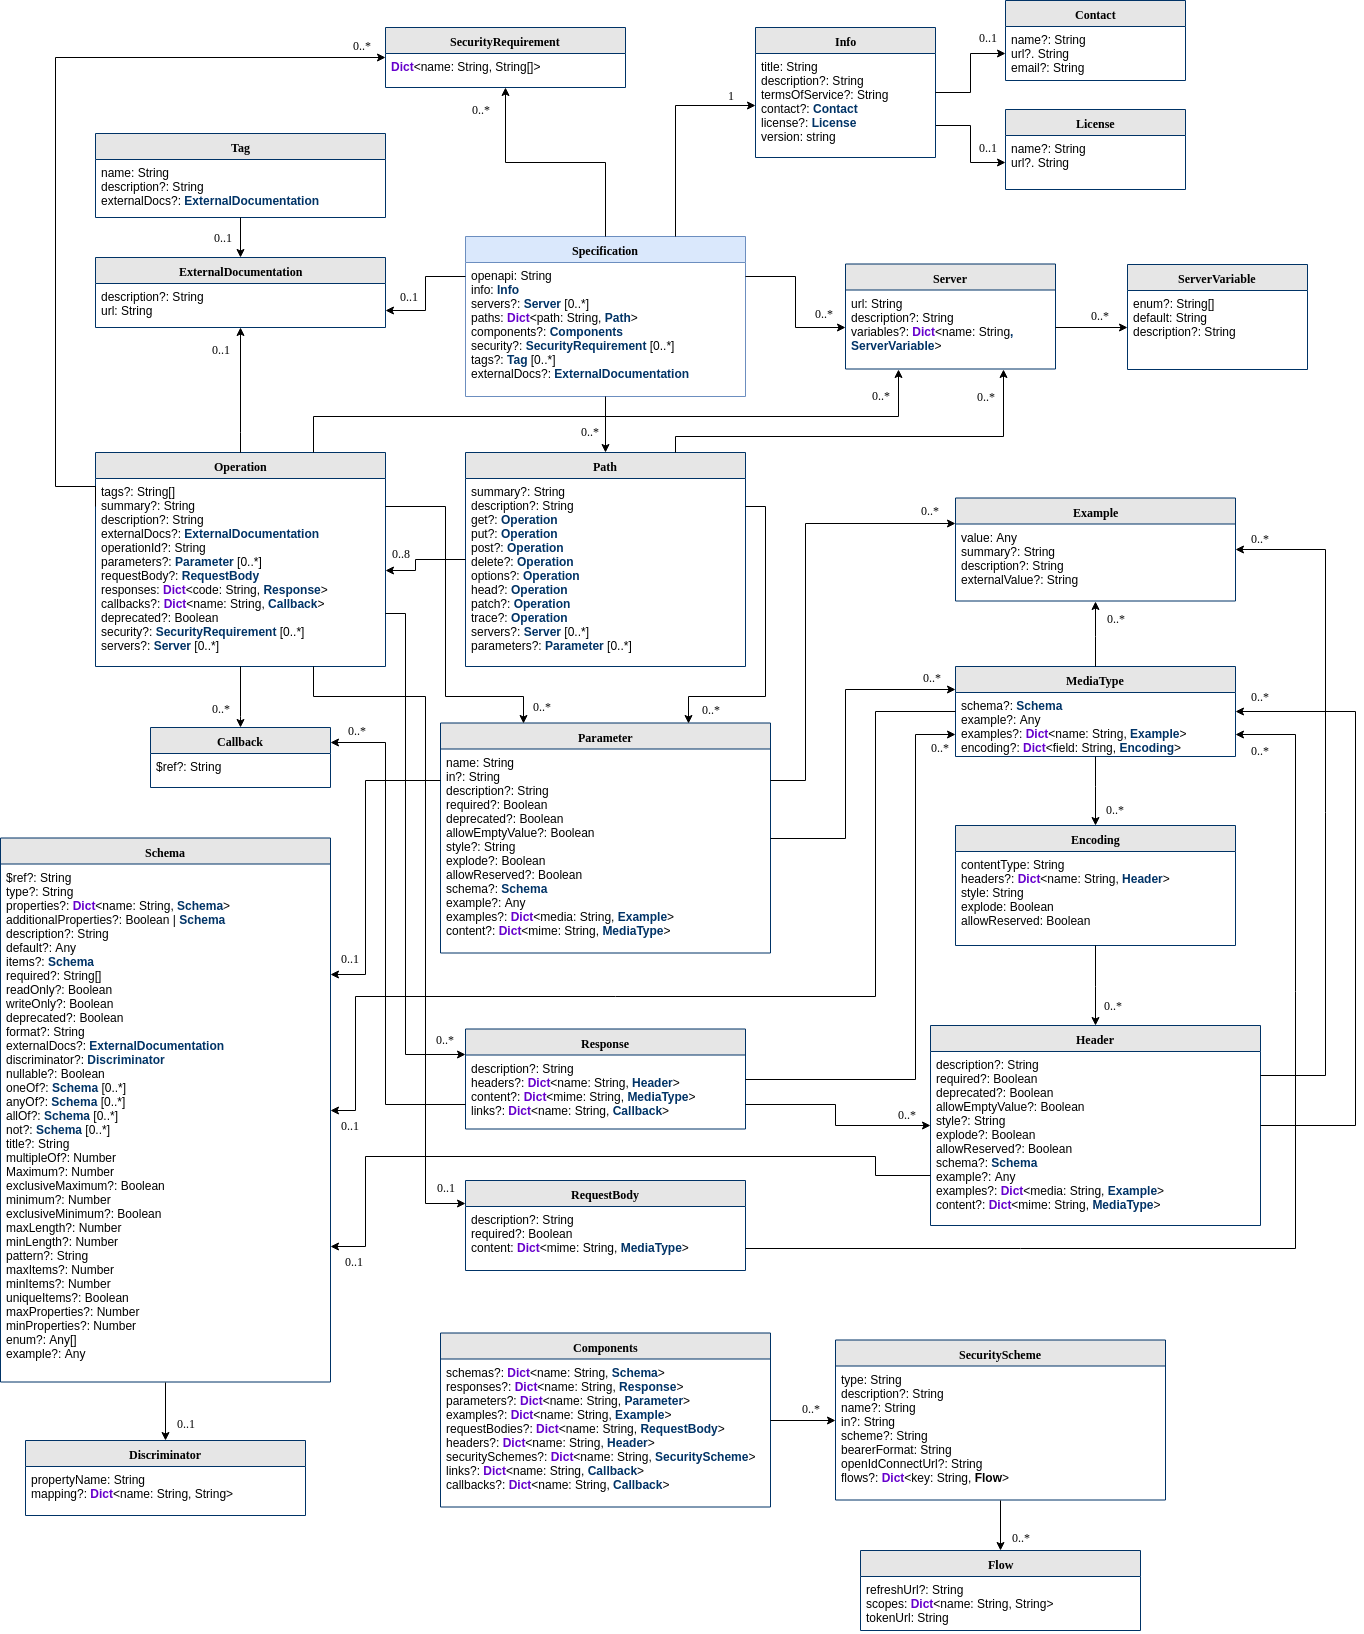
\includegraphics[width=\textwidth,height=\textheight,keepaspectratio]{../images/open-api.png}
  \caption{OpenAPI Metamodell}
  \label{fig:openapi}
\end{figure}

Es wurden ebenfalls zwei weitere Datenmodelle erstellt, die für die im Prototyp festgelegten Ziele benötigt werden. Zunächst wurde ein Modell der JSON-Schema Spezifikation erstellt, welche sich nur in wenigen Divergenzen von der OpenAPI Schema Definition unterscheidet:

\begin{enumerate}
	\item Einige im OpenAPI Schema vorhandene Attribute wie bspw. \lstinline|nullable| oder \lstinline|deprecated| werden nicht unterstützt.
	\item Die \lstinline|type| Angabe kann sowohl ein String wie auch ein String-Array sein.
	\item in \lstinline|$schema| wird zusätzlich ein Link zur verwendeten JSON-Schema Version angegeben. 
\end{enumerate}

Diese Unterschiede müssen bei einer Umwandlung rekursiv aufgelöst werden, da ein Schema weitere verschaltete Schema-Defitionen enthalten kann. Das Modell einer JSON-Schema Definition ist in Abbildung \ref{fig:jsonschema} dargestellt.

\begin{figure}
\centering
  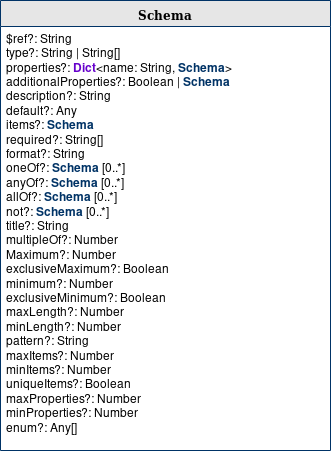
\includegraphics[width=0.5\textwidth]{../images/json-schema.png}
  \caption{JSON-Schema Metamodell}
  \label{fig:jsonschema}
\end{figure}

%------------------------------------------------

\subsection{Architektur}

%------------------------------------------------

\subsection{Vorgehensmodell}
